\documentclass{../../zirkelblatt}

\usepackage{geometry}
\geometry{tmargin=0.5cm,bmargin=0.5cm,lmargin=1cm,rmargin=1cm}

\pagestyle{empty}

\begin{document}

\newcommand{\vorderseite}{
  \begin{minipage}[t][4cm][t]{7.6cm}
    \begin{center}
      \textsf{$\zeta(5)$: eine Zahl, die vielleicht rational ist}
      \vspace{0.6em}
      \tiny

      \scalebox{1.00}{036 927 7551 433 699 2633 136 548 6457 034 168 0570 809 195 0191}

      \scalebox{1.00}{281 197 4192 677 903 8035 897 862 8148 456 004 3106 557 133 3363}

      \scalebox{1.00}{796 203 4146 655 660 9042 800 961 7791 559 708 4183 511 072 1800}

      \scalebox{1.00}{876 448 6628 633 718 0353 598 363 9623 651 288 8898 133 527 6775}

      \scalebox{1.00}{239 827 5032 022 436 8457 664 446 6595 811 599 3917 977 745 0392}

      \scalebox{1.00}{446 439 1966 661 596 6401 620 532 5205 021 519 2267 135 125 6785}

      \scalebox{1.00}{974 869 2860 197 447 9843 200 672 6812 975 309 1990 077 465 6558}

      \scalebox{1.00}{601 526 5737 300 375 6153 268 314 9897 971 935 0398 378 581 3199}

      \scalebox{1.00}{228 848 8642 533 510 4251 602 510 8499 043 464 0294 117 243 2757}

      \scalebox{1.00}{634 150 8162 332 245 6186 499 271 4427 226 461 4113 007 580 8683}
    \end{center}
    \vspace{-0.15cm}
    \centering%
    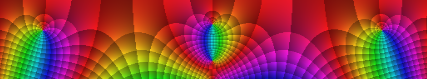
\includegraphics[width=0.95\textwidth]{zeta}%
    \par
  \end{minipage}
}

\newcommand{\rueckseite}{
  \begin{minipage}[t][4cm][t]{7.6cm}
    \phantom{A}
    \vspace{-0.3em}
    \tiny

    Die Zahl~$\zeta(5)$ ist ungefähr 1: $\zeta(5) = 1{,}036\ldots$
    In der Physik kommt sie in quantenmechanischen Modellen von \textbf{Magnetismus}
    vor. Sie ist ein Wert der \textbf{Riemannschen
    $\boldsymbol{\zeta}$-Funktion} mit $\zeta(s) = 1/1^s + 1/2^s + 1/3^s +
    \cdots$. Man vermutet, dass~$\zeta(3), \zeta(5), \zeta(7), \zeta(9),
    \ldots$ alle \textbf{transzendent} sind, also nicht Lösung irgendeiner
    Polynomgleichung mit rationalen Koeffizienten. \textbf{Bewiesen} ist bisher
    aber nur, dass~$\zeta(3)$ und \textbf{mindestens eine} der
    Zahlen~$\zeta(5)$, $\zeta(7)$, $\zeta(9)$ und~$\zeta(11)$ irrational sind.
    Die Werte von~$\zeta$ an allen ganzen Zahlen gehören zu den
    \textbf{Perioden}, einem abzählbaren Zahlbereich, der die algebraischen
    Zahlen, aber auch wichtige transzendente Konstanten wie~$\pi$ und die
    Logarithmen aller algebraischen Zahlen enthält. Man kennt einen
    \textbf{Algorithmus}, der von zwei Perioden entscheiden soll, ob sie gleich
    sind oder nicht. Man \textbf{hofft}, dass dieser stets korrekt arbeitet,
    aber das ist ein \textbf{offenes Problem}.
    \scalebox{0.7}{\begin{minipage}{1.42\textwidth}
    \vspace{-1.3em}
    \begin{align*}
      \zeta(5) &= \frac{1}{294}\pi^5 -\frac{72}{35} \sum_{n=1}^\infty
      \frac{1}{n^5 (e^{2\pi n} -1)}-\frac{2}{35} \sum_{n=1}^\infty \frac{1}{n^5
      (e^{2\pi n} +1)} \\
      \zeta(s) &= \prod\nolimits_p \frac{1}{1 - p^{-s}}
      \qquad\qquad
      \zeta(2n) = (-1)^{n+1} \frac{B_{2n} \cdot (2\pi)^{2n}}{2 \cdot (2n)!}
    \end{align*}\end{minipage}}
  \end{minipage}
}

\vorderseite\hfill\vorderseite
\vfill
\vorderseite\hfill\vorderseite
\vfill
\vorderseite\hfill\vorderseite
\vfill
\vorderseite\hfill\vorderseite
\vfill
\vorderseite\hfill\vorderseite

\newpage

\fontfamily{kurier}\selectfont

\rueckseite\hfill\rueckseite
\vfill
\rueckseite\hfill\rueckseite
\vfill
\rueckseite\hfill\rueckseite
\vfill
\rueckseite\hfill\rueckseite
\vfill
\rueckseite\hfill\rueckseite

\end{document}
